\documentclass[aspectratio=169]{beamer}
\usepackage{ulem}
\usepackage{tikz}
\usepackage{booktabs}
 \usepackage{graphicx,threeparttable,caption}
\usetikzlibrary{shapes,snakes}
\usepackage[beamer,customcolors]{hf-tikz}
\usepackage{nicematrix}
\usepackage{xcolor}
\usepackage{makecell}
\usepackage{array}
\usepackage{csquotes}
\usepackage{csquotes}
\usepackage{minted}
\captionsetup{labelformat=empty,labelsep=none}

\graphicspath{ {./png/} }

\usetikzlibrary{
    arrows,
    arrows.meta,
    shapes,
    positioning,
    shadows,
    trees,
    calc
}

\tikzset{%
    >={Latex[width=2mm,length=2mm]},
    % Specifications for style of nodes:
    plain/.style = {},
    base/.style = {
        plain,
        rectangle, rounded corners, draw=black,
        minimum width=1cm, minimum height=1cm,
        text centered, font=\sffamily\tiny\bfseries,
        fill=white, align=center
    },
    app/.style = {base, ellipse},
    data/.style = {base, fill=gray!30},
    action/.style = {base, circle, fill=red!30},
    note/.style = {app, fill=yellow},
    hl/.style={
    set fill color=red!80!black!40,
    set border color=red!80!black
    }
}


\AtBeginSection[]{
  \begin{frame}
  \vfill
  \centering
  \begin{beamercolorbox}[sep=8pt,center,shadow=true,rounded=true]{title}
    \usebeamerfont{title}\insertsectionhead\par%
  \end{beamercolorbox}
  \vfill
  \end{frame}
}
%\usecolortheme[orchid]{structure}
\usetheme[hideothersubsections]{PaloAlto}
\makeatletter
\patchcmd{\csq@bquote@i}{{#6}}{{\emph{#6}}}{}{}
\makeatother
%\usecolortheme{orchid}
%\usefonttheme{professionalfonts}
\newcommand{\soutthick}[1]{%
   \textcolor{red}{
   \renewcommand{\ULthickness}{1pt}%
      \sout{#1}%
   \renewcommand{\ULthickness}{.4pt}% Resetting to ulem default
   }
}
\newcommand{\centered}[1]{\begin{tabular}{l} #1 \end{tabular}}
\setbeamertemplate{section in toc}[square]
\setbeamertemplate{subsection in toc}[square]
\setbeamertemplate{secion in sidebar}[shaded]
\setbeamertemplate{items}[square]
\setbeamercovered{transparent} 

\title[]{Introduction to Computational Social Science}
\subtitle{Text as data -- does computer understand textual data?}
\author[]{Mikołaj Biesaga\\ \small{\color{blue}{\href{mailto:m.biesaga@uw.edu.pl}{m.biesaga@uw.edu.pl}}}}
\institute{
\includegraphics[width = 4 cm]{uw.png}}
\date{\today}
\begin{document}
\begin{frame}
   \titlepage
\end{frame}

\section[Data]{Data, again}

\begin{frame}
    \frametitle{Structured and Unstructured Data}
    \only<+>{
        \begin{figure}
            
\includegraphics[width = \textwidth]{structured.jpg}
        \end{figure}
    }
    \only<+>{
        \centering
        \begin{columns}[t]
        \begin{column}{.5\textwidth}
            Structured Data:
            \begin{itemize}
                \item can be displayed in rows and columns
                \item numbers, text, dates
                \item requires less storage
                \item easy to manage and analysis
            \end{itemize}
        \end{column}
        \begin{column}{.5\textwidth}
            Unstructured Data:
            \begin{itemize}
                \item can't be displayed in rows and columns
                \item images, audio, video, e-mails, spreadsheets, etc. (fun staff)
                \item requires more storage
                \item extremely hard to manage and analysis
            \end{itemize}
        \end{column}
        \end{columns}
    }
\end{frame}

\begin{frame}
    \frametitle{Data Formats}
    \only<+>{
        Marianna is a 17 years old young lady. Although her main field of interest is physics (especially quantum physics and string theory), she also fancies sports. Her favorite physical activities are fishing and football.
        Marian, on the other hand, is a naughty 15 years old boy who only loves literature, especially Szymborska poems touch his heart.
    }
    \only<+>{
        \textcolor{red}{Marianna} is a \textcolor{blue}{17} years old young lady. Although her main field of interest is \underline{physics} (especially \textbf{quantum physics} and \textbf{string theory}), she also fancies \underline{sport}. Her favorite physical activities are \textbf{fishing} and \textbf{football}.
        \textcolor{red}{Marian}, on the other hand, is a naughty \textcolor{blue}{15} years old boy who only loves \underline{literature}, especially Szymborska \textbf{poems} touches his heart.
    }
    \only<+>{
        \resizebox{\textwidth}{!}{
            \begin{tabular}{l | c | c | c | c | c | c | c | c }
            Name & Sex & Age & Interest A & Interest A1 & Interest A2 & Interest B & Interest B1 & Interest B2\\
            \hline \hline
            Marianna & F & 17 & physics & quantum physics & string theory & sport & fishing & football\\
            Marian & M & 15 & literature & poems & n/a & n/a & n/a & n/a \\
            \end{tabular}}

    }
\end{frame}

\begin{frame}[fragile]{JSON - JavaScript Object Notation}
\begin{minted}[fontsize=\footnotesize]{js}
{   "name": "Marianna",
    "age": 17,
    "interests": [
        {
            "name": "physics",
            "field": [
                "quantum physics",
                "string theory"
            ]
        },
        {
            "name": "sport",
            "field": [
                "fishing",
                "football"
            ]
        }
]}
\end{minted}
\end{frame}

\begin{frame}[fragile]{JSON - JavaScript Object Notation}
\begin{minted}[fontsize=\footnotesize]{js}
{
    "name": "Marian",
    "age": 15,
    "interests": [
        {
            "name": "literature",
            "genre": [
                "poems"
            ]
        }
    ]
}
\end{minted}
\end{frame}

\begin{frame}
    \frametitle{JSON - JavaScript Object Notation}
    \begin{definition}
        \emph{JavaScript Object Notation} is a lightweight text data format that is relatively easy to read for both the human naked eye and computers. Although it derives from JavaScript it is a language-independent data format. JSON is built on two structures: a collection of key-item pairs and an ordered list of values. JSON filenames use .json extension.
    \end{definition}
\begin{definition}
    \emph{JSON Lines} (newline-delimited JSON) is a lightweight text data format that can be processed one record at a time. Each line consists of a JSON. JSON Lines filenames use .jl or .jsonl extensions.
\end{definition}
\end{frame}

\section[Dating]{Ok, Cupid}

\begin{frame}
    \frametitle{What message to write on a dating app?}
    \begin{figure}
        \begin{minipage}{.3\textwidth}
            \vspace{.65cm}
            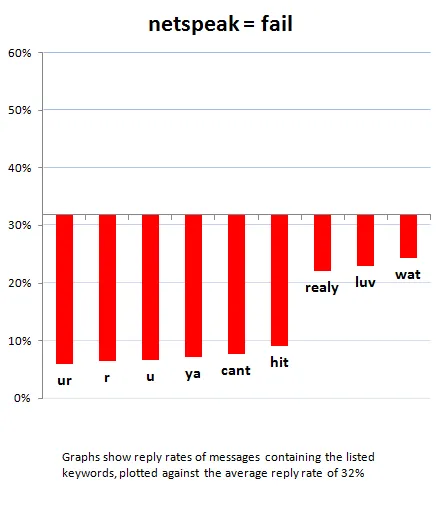
\includegraphics[width = \textwidth]{cupid_1.png}
        \end{minipage}
        \begin{minipage}{.3\textwidth}
            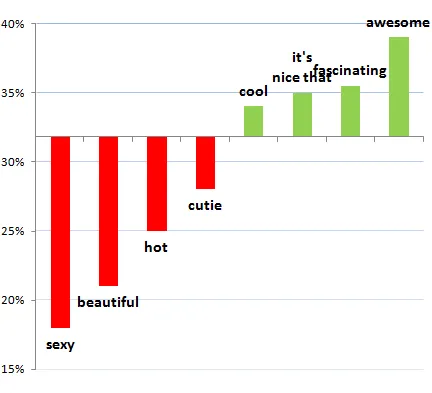
\includegraphics[width = \textwidth]{cupid_2.png}
        \end{minipage}
        \begin{minipage}{.3\textwidth}
            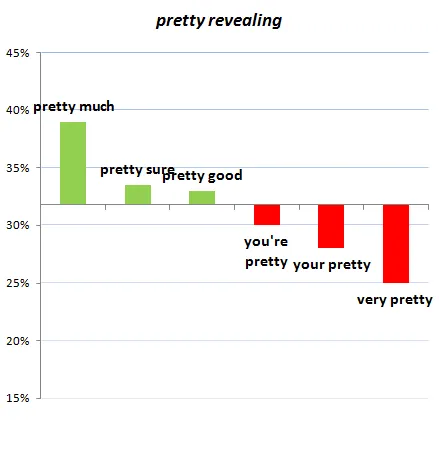
\includegraphics[width = \textwidth]{cupid_3.png}
        \end{minipage}
        \caption*{from \href{https://medium.com/p/2bf680806c72}{\textcolor{blue}{Medium.com}}}
    \end{figure}

\end{frame}

\section[NLP]{Natural Language Processing}

\begin{frame}
    \frametitle{Natural Language Processing}
    \only<+>{
        \begin{definition}
            In a general sense \emph{Natural Language Processing} (NLP) is an analytical approach that uses a set of (usually) computer-based methods to extract meaning, topics, or sentiment from natural language data (written or spoken). In other words, it is a set of computer algorithms that tries to synthesize human language.  \end{definition}
    }
\end{frame}
\begin{frame}
    \frametitle{Sentiment Analysis}
    \only<+>{
        \begin{figure}
            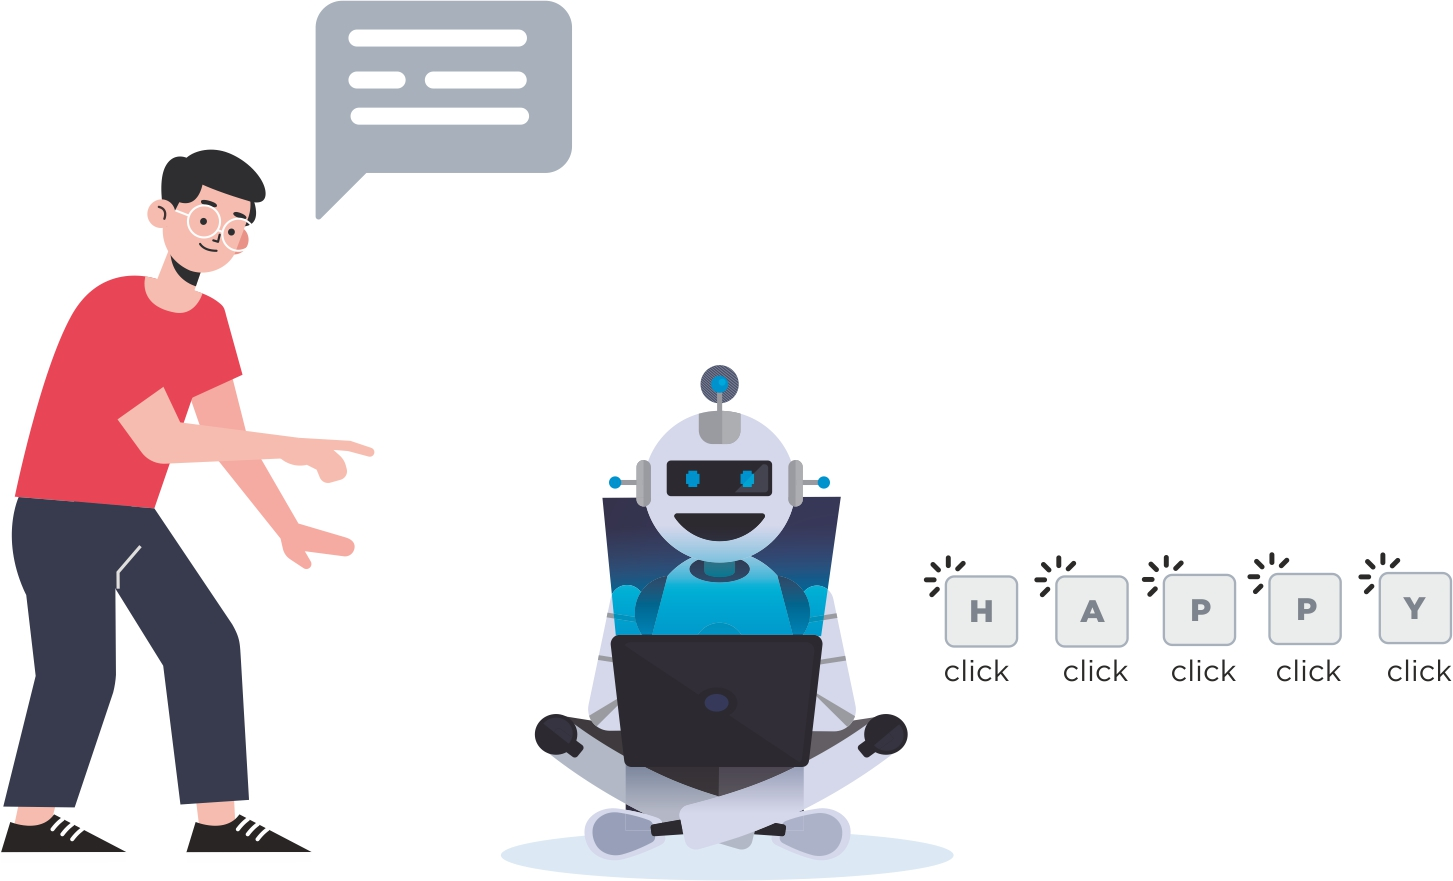
\includegraphics[scale = .7]{png/nlp.jpg}
        \end{figure}
    }
    \only<+>{
        \framesubtitle{Dictionary-based approach}
        \begin{figure}
            \begin{tikzpicture}[>=stealth, text-node/.style={
                rectangle, draw=black, fill=gray!20, text centered, rounded corners}]
                \node[text-node, text width = 3cm] at (0,0) {This movie was so good -- I couldn't stop thinking about it afterward.};
                \node[text-node, text width = 3cm] at (3,4) {The actors were great, but the story was boring and predictable.};
                \node[text-node, text width = 3cm] at (4,2) {It looked amazing, but the characters didn't feel real.};
                \node[text-node, text width = 3cm] at (9,4) {I loved the action scenes; they kept me hooked the whole time.};
                \node[text-node, text width = 3cm] at (8,0) {It felt like the movie was trying too hard to be deep, but it just ended up confusing.};
            \end{tikzpicture}
        \end{figure}
    }
    \only<+>{
        \framesubtitle{Preprocessing}
        \begin{figure}
            \begin{tikzpicture}[>=stealth, text-node/.style={
                rectangle, draw=black, fill=gray!20, text centered, rounded corners, font=\small}]
                \node[text-node, text width = 3cm] (text) at (0,0) {This move was so good -- I couldn't stop thinking about it afterward.};
                \node [text-node, text width = 1.5cm] (token) at (4,0) {This\\ movie\\ was\\ so\\ good\\ --\\ I\\ couldn't\\ stop\\ thinking\\ about\\ it\\ afterward.};
                \node [text-node, text width = 1.5cm] (lemma) at (7,0) {this\\ movie\\ be\\ so\\ good\\ --\\ i\\ cannot\\ stop\\ think\\ about\\ it\\ afterward};
                \node [text-node, text width = 1.5cm] (stop) at (10,0) {\phantom{this}\\ movie\\ be\\ so\\ good\\ \phantom{--}\\ \phantom{I}\\ cannot\\ stop\\ think\\ \phantom{about}\\ \phantom{it}\\ afterward};
                \node at (0,-3.5) {Text};
                \node at (4,-3.5) {Tokenization};
                \node at (7,-3.5) {Lemmatization};
                \node at (10,-3.5) {Stop words};
                \draw [->] (1.7, 0) -- (3,0);
                \draw [->] (5,0) -- (6,0);
                \draw [->] (8,0) -- (9,0);
            \end{tikzpicture}
        \end{figure}
    }
    \only<+>{
        \begin{figure}
            \begin{tikzpicture}[>=stealth, text-node/.style={
                rectangle, draw=black, fill=gray!20, text centered, rounded corners, font=\small}]
                \node [text-node, text width = 1.5cm] (stop) at (0,0) {\phantom{this}\\ movie\\ be\\ so\\ good\\ \phantom{--}\\ \phantom{I}\\ cannot\\ stop\\ think\\ \phantom{about}\\ \phantom{it}\\ afterward};
                \node [text-node, text width = 1.5cm] (stop) at (4,0) {\phantom{this}\\ movie\\ be\\ so\\ \colorbox{green!20}{good}\\ \phantom{--}\\ \phantom{I}\\ cannot\\ stop\\ think\\ \phantom{about}\\ \phantom{it}\\ afterward};
                \node [text-node, text width = 1.5cm, fill = green!20] (stop) at (8,0) {\phantom{this}\\ movie\\ be\\ so\\ good\\ \phantom{--}\\ \phantom{I}\\ cannot\\ stop\\ think\\ \phantom{about}\\ \phantom{it}\\ afterward};
                \node at (8,-3.5) {$sentiment = +.125$};
                \draw [->] (1, 0) -- (3,0);
                \draw [->] (5, 0) -- (7,0);
            \end{tikzpicture}
        \end{figure}
    }
    \only<+>{
        \framesubtitle{Dictionary-based approach}
        \begin{figure}
            \begin{tikzpicture}[>=stealth, text-node/.style={
                rectangle, draw=black, fill=gray!20, text centered, rounded corners}]
                \node[text-node, text width = 3cm, fill = green!20] at (0,0) {This movie was so good -- I couldn't stop thinking about it afterward.};
                \node[text-node, text width = 3cm, fill = red!20] at (3,4) {The actors were great, but the story was boring and predictable.};
                \node[text-node, text width = 3cm, fill = green!20] at (4,2) {It looked amazing, but the characters didn't feel real.};
                \node[text-node, text width = 3cm, fill = green!20] at (9,4) {I loved the action scenes; they kept me hooked the whole time.};
                \node[text-node, text width = 3cm, fill = red!20] at (8,0) {It felt like the movie was trying too hard to be deep, but it just ended up confusing.};
            \end{tikzpicture}
        \end{figure}
    }
    \only<+>{
        \framesubtitle{Machine Learning approach}
        \begin{figure}
            \begin{tikzpicture}[>=stealth, text-node/.style={
                rectangle, draw=black, fill=gray!20, text centered, rounded corners, font=\small}]
                \node[text-node, text width = 3cm] at (0,0) {This move was so good -- I couldn't stop thinking about it afterward.};
                \draw[fill = black] (4,-1) rectangle (6,1);
                \node[text-node, text width = 3cm, fill = green!20] at (10,0) {This move was so good -- I couldn't stop thinking about it afterward.};
                \draw [->] (1.7,0) -- (3.9,0);
                \draw [->] (6.1,0) -- (8.3,0);
                \node at (0,-2.5) {Text};
                \node at (5,-2.5) {Black box};
                \node at (10,-2.5) {$sentiment = +.93$};
            \end{tikzpicture}
        \end{figure}

    }
\end{frame}
\begin{frame}
    \frametitle{Topic Modeling}
    \only<+>{
        \begin{figure}
        \begin{tikzpicture}[>=stealth, scale = .5, small/.style={
            % The shape:
            rectangle,
            % The size:
            minimum size=.75cm,
            % The border
            thick, draw=black,
            % The filling
            fill=white}]
        \foreach \x/\y in {0/0,2/0,8/0}{
          \draw [fill = yellow!30] (\x + 0,0 - \y) rectangle (\x + 1.5,2 - \y);
          \draw (\x + .2,1.4 - \y) rectangle (\x + 1.3,1.9 - \y);
          \foreach \z in {.2,.3,...,1.3}{
            \draw (\x + .2,\z - \y) -- (\x + 1.3,\z - \y);
          }
        }
        \foreach \x/\y in {12/0,6/0,10/0}{
          \draw [fill = red!30] (\x + 0,0 - \y) rectangle (\x + 1.5,2 - \y);
          \draw (\x + .2,1.4 - \y) rectangle (\x + 1.3,1.9 - \y);
          \foreach \z in {.2,.3,...,1.3}{
            \draw (\x + .2,\z - \y) -- (\x + 1.3,\z - \y);
          }
        }
        \foreach \x/\y in {4/0}{
          \draw [fill = green!30] (\x + 0,0 - \y) rectangle (\x + 1.5,2 - \y);
          \draw (\x + .2,1.4 - \y) rectangle (\x + 1.3,1.9 - \y);
          \foreach \z in {.2,.3,...,1.3}{
            \draw (\x + .2,\z - \y) -- (\x + 1.3,\z - \y);
          }
        }
        \foreach \x/\y in {3/4, 3/4.3, 3/4.6}{
          \draw [fill = yellow!30] (\x + 0,0 - \y) rectangle (\x + 1.5,2 - \y);
          \draw (\x + .2,1.4 - \y) rectangle (\x + 1.3,1.9 - \y);
          \foreach \z in {.2,.3,...,1.3}{
            \draw (\x + .2,\z - \y) -- (\x + 1.3,\z - \y);
          }
        }
        \foreach \x/\y in {9/4, 9/4.3, 9/4.6}{
          \draw [fill = red!30] (\x + 0,0 - \y) rectangle (\x + 1.5,2 - \y);
          \draw (\x + .2,1.4 - \y) rectangle (\x + 1.3,1.9 - \y);
          \foreach \z in {.2,.3,...,1.3}{
            \draw (\x + .2,\z - \y) -- (\x + 1.3,\z - \y);
          }
        }
        \foreach \x/\y in {6/4}{
          \draw [fill = green!30] (\x + 0,0 - \y) rectangle (\x + 1.5,2 - \y);
          \draw (\x + .2,1.4 - \y) rectangle (\x + 1.3,1.9 - \y);
          \foreach \z in {.2,.3,...,1.3}{
            \draw (\x + .2,\z - \y) -- (\x + 1.3,\z - \y);
          }
        }
        \draw (.75,0) [->] -- (3.65, -2);
        \draw (2.75,0) [->] -- (3.75, -2);
        \draw (8.75,0) [->] -- (3.85, -2);
        \draw (4.75,0) [->] -- (6.75, -2);
        \draw (6.75,0) [->] -- (9.65, -2);
        \draw (10.75,0) [->] -- (9.75, -2);
        \draw (12.75,0) [->] -- (9.85, -2);
    
        \draw [fill = yellow!30] (3, -8.6) rectangle (4.5, -6.6);
        \draw [fill = red!30] (9, -8.6) rectangle (10.5, -6.6);
    
        \draw (3.75, -4.8) -- ++(270:1.6) -- ++(0:6) -- ++(90:1.6);
    
        \node at (16,1) {Corpus};
        \node at (16,-3) {Separated Topics};
        \node at (16,-7.3) {Identified Narratives};
    
        \end{tikzpicture}
    \end{figure}
    }
    \only<+>{
        \begin{figure}
            \begin{tikzpicture}[>=stealth, text-node/.style={
                rectangle, draw=black, fill=gray!20, text centered, rounded corners}]
                \node[text-node, text width = 3cm] (T1) at (0,0) {Fear of failure leads to failure.};
                \node[text-node, text width = 3cm] (T2) at (3,4) {If we do not face our fears, our fears will chase us forever.};
                \node[text-node, text width = 3cm] (T3) at (4,1.5) {Do not fear to love for the first time.};
                \node[text-node, text width = 3cm] (T4) at (9,4) {We do not need to explain our love. We only need to show it.};
                \node[text-node, text width = 3cm] (T5) at (8,0) {Love yourself first because this is the person you are going to spend the rest of your life with.};
                \node at (-2.25, 0) {T1 = };
                \node at (.75, 4) {T2 = };
                \node at (1.75,1.5) {T3 = };
                \node at (6.75,4) {T4 = };
                \node at (5.75,0) {T5 = };
            \end{tikzpicture}
        \end{figure}
    }
    \only<+>{
        \begin{enumerate}
            \item Corpus preprocessing: Tokenization $=>$ Lemmatization $=>$ Stop
            words removal.
            \item Vectorization of the text (text embeddings).
            \item Training a model.
            \item Testing the model.
        \end{enumerate}
    }
    \only<+>{
        \framesubtitle{What is a vector?}
        \begin{definition}{}
            In mathematics and physics, \emph{vector} is a term that refers to
            quantities that cannot be expressed by a single number (a scalar),
            or to elements of some vector spaces.
        \end{definition}
    }
    \only<5,6>{
        \framesubtitle{What is a vector?}
        \begin{figure}
            \begin{tikzpicture}
                \draw[->, thick] (0, 0) --++ (0: 6cm) node [below] {x};
                \draw[->, thick] (0, 0) --++ (90: 6cm) node [left] {y};
                \draw node at (4cm,3cm) {\LARGE.};
                \draw<5> node at (4,3) [right] {A};
                \foreach \x in {1,...,5}{
                    \draw (\x, -.05) node [below] {\x} -- (\x, .05);
                    \draw (-.05, \x) node [left] {\x} -- (.05, \x);
                }
                \draw<6> node at (4,3) [right]{A(4,3)};
                \draw<6> [dashed, thin, gray] (4,0) -- (4,3);
                \draw<6> [dashed, thin, gray] (0,3) -- (4,3);
                \draw<6> node at (4,3) [right]{A(4,3)};
            \end{tikzpicture}
    \end{figure}
    }
    \only<7>{
        \framesubtitle{Bag of words}
        \begin{figure}
            \begin{tikzpicture}[>=stealth, text-node/.style={
                rectangle, draw=black, fill=gray!20, text centered, rounded corners}]
                \node[text-node, text width = 3cm] (T1) at (0,0) {fear \phantom{of} failure lead \phantom{to} failure};
                \node[text-node, text width = 3cm] (T2) at (3,4) {\phantom{If} \phantom{we} do not face \phantom{our} fear \phantom{our} fear be chase \phantom{us} forever};
                \node[text-node, text width = 3cm] (T3) at (4,1.5) {do not fear \phantom{to} love \phantom{for} \phantom{the} first time};
                \node[text-node, text width = 3cm] (T4) at (9,4) {\phantom{We} do not need \phantom{to} explain \phantom{our} love \phantom{We} only need \phantom{to} show \phantom{it}};
                \node[text-node, text width = 3cm] (T5) at (8,0) {love \phantom{yourself} first \phantom{because} \phantom{this} be \phantom{the} person \phantom{you} be go \phantom{to} spend \phantom{the} rest \phantom{of} \phantom{your} life \phantom{with}};
                \node at (-2.25, 0) {T1 = };
                \node at (.75, 4) {T2 = };
                \node at (1.75,1.5) {T3 = };
                \node at (6.75,4) {T4 = };
                \node at (5.75,0) {T5 = };
            \end{tikzpicture}
        \end{figure}
    }
    \only<8>{
        \framesubtitle{Bag of words}
        \begin{figure}
            \begin{tikzpicture}[>=stealth, text-node/.style={
                rectangle, draw=black, fill=gray!20, text centered, rounded corners}]
                \node[text-node, text width = 3cm] (T1) at (0,0) {\colorbox{yellow}{fear} \phantom{of} failure lead \phantom{to} failure};
                \node[text-node, text width = 3cm] (T2) at (3,4) {\phantom{If} \phantom{we} do not face \phantom{our} \colorbox{yellow}{fear} \phantom{our} \colorbox{yellow}{fear} be chase \phantom{us} forever};
                \node[text-node, text width = 3cm] (T3) at (4,1.5) {do not \colorbox{yellow}{fear} \phantom{to} \colorbox{blue}{love} \phantom{for} \phantom{the} first time};
                \node[text-node, text width = 3cm] (T4) at (9,4) {\phantom{We} do not need \phantom{to} explain \phantom{our} \colorbox{blue}{love} \phantom{We} only need \phantom{to} show \phantom{it}};
                \node[text-node, text width = 3cm] (T5) at (8,0) {\colorbox{blue}{love} \phantom{yourself} first \phantom{because} \phantom{this} be \phantom{the} person \phantom{you} be go \phantom{to} spend \phantom{the} rest \phantom{of} \phantom{your} life \phantom{with}};
                \node at (-2.25, 0) {T1 = };
                \node at (.75, 4) {T2 = };
                \node at (1.75,1.5) {T3 = };
                \node at (6.75,4) {T4 = };
                \node at (5.75,0) {T5 = };
            \end{tikzpicture}
        \end{figure}
    }
    \only<9>{
        \framesubtitle{How to convert text into a vector?}
        \begin{figure}
            \begin{tikzpicture}
                \draw[->, thick] (0, 0) --++ (0: 6cm) node [below] {fear};
                \draw[->, thick] (0, 0) --++ (90: 6cm) node [left] {love};
                \foreach \x in {1,...,5}{
                    \draw (\x, -.05) node [below] {\x} -- (\x, .05);
                    \draw (-.05, \x) node [left] {\x} -- (.05, \x);
                }
                \node at (1,0) {\LARGE .};
                \node at (1,0) [above] {\textcolor{yellow}{T1}};
                \node at (2,0) {\LARGE .};
                \node at (2,0) [above] {\textcolor{yellow}{T2}};
                \node at (0,1) {\LARGE .};
                \node at (0,1) [above right] {\textcolor{blue}{T4}};
                \node at (0,1) [below right] {\textcolor{blue}{T5}};
                \node at (1,1) {\LARGE .};
                \node at (1,1) [above right] {\textcolor{green}{T3}};
            \end{tikzpicture}
    \end{figure}
    }
    \only<10>{
        \framesubtitle{Cosine similarity}
        \begin{figure}
            \begin{tikzpicture}
                \draw[->, thick] (0, 0) --++ (0: 6cm) node [below] {x};
                \draw[->, thick] (0, 0) --++ (90: 6cm) node [left] {y};
                \foreach \x in {1,...,5}{
                    \draw (\x, -.05) node [below] {\x} -- (\x, .05);
                    \draw (-.05, \x) node [left] {\x} -- (.05, \x);
                }
                \draw (0,0) --++ (30:4) node [above] {$T_n(x_{n}, y_{n})$};
                \draw (0,0) --++ (75:5) node [above] {$T_{n+1}(x_{n+1}, y_{n+1})$};
                \draw (0,0) --++ (30:4) node {\LARGE .};
                \draw (0,0) --++ (75:5) node {\LARGE .};
                \draw (0,0) ++(30:1) arc (30:75:1) node [xshift = .2cm, yshift = -.4cm] {$\alpha$};

            \end{tikzpicture}
        \end{figure}
    }
    \only<11>{
        \framesubtitle{Cosine similarity}
        \begin{figure}
            \begin{tikzpicture}[help lines/.style={black!50,very thin}]
                \foreach \x in {-360,-270,-180,-90,+90,+180,+270,+360} \draw ({\x/90},-0.05) -- ({\x/90},0.05) node[below] {$\x^\circ$};
                \foreach \y in {-1,1} \draw (-0.05,\y) -- (0.05, \y) node [left] {$\y$};
                \draw[<->,thick] (-5,0)--(5,0) node[right] {$x$};
                \draw[<->,thick] (0,-2.25)--(0,2.25) node[above] {$y$};
                \draw[very thick,color=black] plot [domain={-360/90}:{360/90},smooth] (\x,{cos(90*\x)});
            \end{tikzpicture}
        \end{figure}
    }
    \only<12>{
        \framesubtitle{Cosine similarity}
        \begin{definition}{}
            In data analysis, \emph{cosine similarity} is a measure of similarity
            between two non-zero vectors defined in an inner product space.
            Cosine similarity is the cosine of the angle between the vectors;
            that is, it is the dot product of the vectors divided by the product
            of their lengths. It follows that the cosine similarity does not
            depend on the magnitudes of the vectors, but only on their angle.
            The cosine similarity always belongs to the interval [−1,1].  For
            example, two proportional vectors have a cosine similarity of 1, two
            orthogonal vectors have a similarity of 0, and two opposite vectors
            have a similarity of -1. 
       \end{definition}
    }
    \only<13>{
        \begin{figure}
            \begin{tikzpicture}
                \draw[->, thick] (0, 0) --++ (0: 6cm) node [below] {x};
                \draw[->, thick] (0, 0) --++ (90: 6cm) node [left] {y};
                \foreach \x in {1,...,5}{
                    \draw (\x, -.05) node [below] {\x} -- (\x, .05);
                    \draw (-.05, \x) node [left] {\x} -- (.05, \x);
                }
                \draw (0,0) ++ (30:4) node {\textcolor{blue}{\tiny o}};
                \draw (0,0) ++ (32:4) node {\textcolor{blue}{\tiny o}};
                \draw (0,0) ++ (28:3.9) node {\textcolor{blue}{\tiny o}};
                \draw (0,0) ++ (30:3.5) node {\textcolor{blue}{\tiny o}};
                \draw (0,0) ++ (35:4) node {\textcolor{blue}{\tiny o}};
                \draw (0,0) ++ (28:3.8) node {\textcolor{blue}{\tiny o}};
                \draw (0,0) ++ (30:3.9) node {\textcolor{blue}{\tiny o}};
                \draw (0,0) ++ (34:3.8) node {\textcolor{blue}{\tiny o}};
                \draw (0,0) ++ (32:3.9) node {\textcolor{blue}{\tiny o}};
                \draw (0,0) ++ (327:3.5) node {\textcolor{blue}{\tiny o}};
                \draw (0,0) ++ (35:4.2) node {\textcolor{blue}{\tiny o}};
                \draw (0,0) ++ (32:3.8) node {\textcolor{blue}{\tiny o}};
                \draw (0,0) ++ (75:5) node {\textcolor{yellow}{\tiny x}};
                \draw (0,0) ++ (80:4.8) node {\textcolor{yellow}{\tiny x}};
                \draw (0,0) ++ (76:4.9) node {\textcolor{yellow}{\tiny x}};
                \draw (0,0) ++ (72:5.1) node {\textcolor{yellow}{\tiny x}};
                \draw (0,0) ++ (76:5) node {\textcolor{yellow}{\tiny x}};
                \draw (0,0) ++ (82:4.6) node {\textcolor{yellow}{\tiny x}};
                \draw (0,0) ++ (76:5.2) node {\textcolor{yellow}{\tiny x}};
                \draw (0,0) ++ (73:5.1) node {\textcolor{yellow}{\tiny x}};
                \draw (0,0) ++ (45:1) node {\textcolor{green}{\tiny *}};
                \draw (0,0) ++ (46:.9) node {\textcolor{green}{\tiny *}};
                \draw (0,0) ++ (47:1.1) node {\textcolor{green}{\tiny *}};
                \draw (0,0) ++ (45:1.2) node {\textcolor{green}{\tiny *}};
                \draw (0,0) ++ (44:.9) node {\textcolor{green}{\tiny *}};
                \draw (0,0) ++ (42:.8) node {\textcolor{green}{\tiny *}};
                \draw (0,0) ++ (48:1.1) node {\textcolor{green}{\tiny *}};
                \draw (0,0) ++ (47:1) node {\textcolor{green}{\tiny *}};

            \end{tikzpicture}

        \end{figure}
    }
    \only<14>{
        \framesubtitle{Output}
        \scriptsize
        For example, imagine you have the following set of sentences (in real-world we would operate on documents that contain multiple sentences).

        \begin{itemize}
            \item I like to eat broccoli and bananas.
            \item I ate a banana and spinach smoothie for breakfast.
            \item Chinchillas and kittens are cute.
            \item My sister adopted a kitten yesterday.
            \item Look at this cute hamster munching on a piece of broccoli.
        \end{itemize}

        The LDA model returns more or less the following information about the probability to belong each sentence to a topic.
        
        \begin{itemize}
            \item Sentences 1 and 2: 100\% Topic A
            \item Sentences 3 and 4: 100\% Topic B
            \item Sentence 5: 60\% Topic A, 40\% Topic B
        \end{itemize}

        And the most representative words for a topic.
        
        \begin{itemize}
            \item Topic A: 30\% broccoli, 15\% bananas, 10\% breakfast, 10\% munching, etc. (at which point, you could interpret topic A to be about food)
            \item Topic B: 20\% chinchillas, 20\% kittens, 20\% cute, 15\% hamster, etc. (at which point, you could interpret topic B to be about cute animals)
        \end{itemize}

    }
\end{frame}


\begin{frame}
    \frametitle{For the class in two weeks}
    \begin{itemize}
        \item Biesaga, M., Domaradzka, A., Roszczyńska-Kurasińska, M., Talaga,
        S., \& Nowak, A. (2023). The effect of the pandemic on European
        narratives on smart cities and surveillance. Urban Studies,
        004209802211383. \href{https://doi.org/10.1177/00420980221138317}{\textcolor{blue}{https://doi.org/10.1177/00420980221138317}}.
    \end{itemize}
\end{frame}
\end{document}
